\chapter{Groups}

\epigraph[author={Mark Armstrong}, source={Groups and Symmetry}]{Numbers measure quantity, groups measure symmetry}\SubIndex{Armstrong, Mark}

\epigraph[author={Henri Poincar\'e}]{The theory of groups is, as it were, the whole of mathematics stripped of its matter 
and reduced to pure form.}\SubIndex{Poincar\'e, Henri}

\section{Transformation groups}

Take a set \(X\), which could be a set of points in the plane, or a set of numbers, or a collection of various geometric figures, or the set of books in a library, or any other set of any sort of things.
A \emph{transformation}\define{transformation} \(f\) of \(X\) associates to each element \(x\) of \(X\) some element \(f(x)\) also from \(X\).

\begin{example}
Take a square \(X\) in the plane, and rotate it around its centre by a right angle.
Each point \(p\) of \(X\) is rotated into some point \(f(p)\).
Note that the centre point of the square is ``fixed'', i.e. rotated into itself.
\end{example}
\begin{example}
Take any set \(X\).
The \emph{identity transformation}\define{transformation!identity}\define{identity transformation} is the transformation that leaves every point of \(X\) where it is: \(f(x)=x\).
\end{example}
\begin{example}
Shuffle a deck of cards.
If \(X\) is the set of cards, the shuffle is a transformation \(f\) of \(X\).
\end{example}

Two maps \(f \colon X \to Y\) and \(g \colon Y \to X\) between sets are \emph{inverses}\define{inverse} if \(f(g(x))=x\) and \(g(f(x))=x\) for any element \(x\) of \(X\).
In other words, \(f \circ g\) and \(g \circ f\) are both the identity transformation.
Recall that a map \(f\) is \emph{invertible}\define{invertible!transformation}\define{transformation!invertible}, also called a \emph{bijection}\define{bijection} or a \emph{permutation}\define{permutation} if it has an inverse.
A bijection transformation is a \emph{permutation}.\define{permutation}

\begin{problem}{groups:bijection}
A map \(f \colon X \to Y\) of a set \(X\) is \emph{injective}\define{injective} (also called \emph{one-to-one}\define{one-to-one}) if \(f(p)=f(q)\) only when \(p=q\).
It is \emph{surjective}\define{surjective} (also called \emph{onto}\define{onto}) if every element \(y\) of \(Y\) has the form \(y=f(x)\) for some element \(x\) of \(X\).
Prove that a map is a bijection just when it is injective and surjective.
\end{problem}

\begin{problem}{groups:bijection.finite}
Prove that a transformation \(f\) of a \emph{finite} set \(X\) is injective just when it is surjective, and hence just when it is a bijection.
\end{problem}
\begin{answer}{groups:bijection.finite}
Denote by \(\cardinality{S}\) the number of elements in a set \(S\).
We use the basic fact that if \(S \subseteq T\) is a subset of a finite set \(T\), then \(\cardinality{S} \le \cardinality{T}\), with equality just when \(S=T\).
The image of \(f\) is \(f(X) \subseteq X\), equality just when \(f\) is surjective, i.e. just when \(\cardinality{f(X)}=\cardinality{X}\).
Each element maps somewhere, i.e. lies in \(f^{-1}(x)\) for some \(x \in f(X)\):
\[
\cardinality{X} = \sum_{x \in f(X)} \cardinality{f^{-1}\set{x}}
\ge \sum_{x \in f(X)} 1 = \cardinality{f(X)},
\]
with equality, i.e. \(f\) surjective, just when \(f^{-1}\set{x}\) has one element for every \(x \in f(X)\), i.e. just when \(f\) is injective.
\end{answer}

\begin{problem}{groups:bijection.inverse}
Prove that a bijection \(f\) has a unique inverse.
\end{problem}
The inverse of a bijection \(f\) is denoted \(f^{-1}\).

A \emph{transformation group}\define{group!transformation}\define{transformation!group} \(G\) on a set \(X\) is a nonempty collection of permutations of \(X\) so that 
\begin{enumerate}
\item 
if \(f\) and \(g\) are in \(G\) then \(f \circ g\) is in \(G\).
\item
if \(f\) is in \(G\) then \(f^{-1}\) is also in \(G\).
\end{enumerate}

\begin{example}
Take \(X\) the Euclidean plane.
Every rotation of the plane around the origin is by some angle, say \(\theta\).
Conversely, every angle \(\theta\) is the angle of some rotation around the origin.
So angles form a transformation group \(G\), the group of rotations of the plane \(X\) around the origin.
\end{example}
\begin{example}
Take \(X\) to be three dimensional Euclidean space.
Take a line \(\ell\) through the origin, with a chosen direction along that line.
Hold the line in your hand, so that your thumb points up the chosen direction.
Then your figures curl around the line in a certain direction.
In additional, take an angle \(\theta\), and rotate the whole space \(X\) around in the direction of your fingers, by the angle \(\theta\).
Every rotation of Euclidean space \(X\) arises in this way.
(If you change the choice of direction to point your thumb, but keep the same axis of rotation \(\ell\), then you change \(\theta\) to \(-\theta\).)
When you compose a rotation with another rotation, the result is yet a third rotation.
The rotations of Euclidean space form a transformation group \(G\).
\end{example}
\begin{example}
Take \(X\) to be the real number line. 
Given any real number \(t\), we can define a transformation \(f(x)=x+t\).
In this way, the real numbers \(t\) are associated to the elements of a group \(G\) of transformations of the real number line.
\end{example}
\begin{example}
A \emph{rigid motion} of Euclidean space is a transformation that preserves distances.
For example, rotations, mirror reflections: \((x,y) \mapsto (x,-y)\), and translations \((x,y) \mapsto (x+x_0,y+y_0)\) are rigid motions of the plane.
The rigid motions form a transformation group.
\end{example}
\begin{example}
Take a geometric figure \(X\) in the plane, or in space.
A rigid motion preserving \(X\) is a \emph{symmetry} of \(X\); the symmetries of a figure constitute a transformation group.
For example, if \(X\) is a square, every symmetry permutes the corners somehow, and we can easily see these symmetries:
\begin{center}
\documentclass[tikz]{standalone}
\usepackage{xparse}
\usetikzlibrary{positioning}
\colorlet{curveZero}{gray!75}
\colorlet{curveOne}{blue!60}
\colorlet{curveTwo}{brown!50!gray}
\colorlet{curveThree}{green!40!gray}
\colorlet{curveFour}{red!50!gray}
\NewDocumentCommand\DrawDotInPlot{O{}mmO{}}%
{%
\fill[gray!20,draw=gray] (axis cs:{#2},{#3}) circle (1.3pt) node[above,black,#4] {\(#1\)};%
}%
\NewDocumentCommand\DrawDot{O{}mmO{}}%
{%
\fill[gray!20,draw=gray] ({#2},{#3}) circle (1.3pt) node[above,black,#4] {\(#1\)};%
}%
\NewDocumentCommand\DrawNode{O{}m}%
{%
\fill[gray!20,draw=gray] (#2) circle (1.3pt) node[above,black] {\(#1\)};%
}%
\colorlet{axisColor}{gray!50}
\tikzstyle{shapeZero}=[fill=curveZero,opacity=.4]
\tikzstyle{shapeOne}=[fill=curveOne,opacity=.4]
\tikzstyle{shapeTwo}=[fill=curveTwo,opacity=.4]
\tikzstyle{shapeThree}=[fill=curveThree,opacity=.4]
\tikzstyle{groupElementLabel}=[minimum size=2.4em]
\tikzstyle{groupElement}=[minimum size=2.4em,shapeZero,draw=curveZero]
\tikzstyle{cosetOne}=[minimum size=2.4em,shapeOne,draw=curveOne]
\tikzstyle{cosetTwo}=[minimum size=2.4em,shapeTwo,draw=curveTwo]


\newcounter{squareBoxCounter}
\begin{document}
\setcounter{squareBoxCounter}{0}
\NewDocumentCommand\sqrbox{mmmm}{%
\stepcounter{squareBoxCounter}%
\begin{scope}[xshift=\thesquareBoxCounter in]%
\fill[shapeZero,draw=curveZero] (0,0) rectangle (1,1);%
\node[below left=-1.3mm and -1.3mm] at (0,0) {#1};%
\node[above left=-1.3mm and -1.3mm] at (0,1) {#2};%
\node[above right=-1.3mm and -1.3mm] at (1,1) {#3};%
\node[below right=-1.3mm and -1.3mm] at (1,0) {#4};%
\end{scope}}%
\begin{tikzpicture}[scale=.5]%
\sqrbox{1}{2}{3}{4}%
\sqrbox{4}{1}{2}{3}%
\sqrbox{1}{4}{3}{2}%
\end{tikzpicture}%
\end{document}
\end{center}
The symmetry group of a non-isosceles triangle consists just of the identity transformation.
For an isosceles, but not equilateral, triangle, the symmetry group is the identity transformation and the reflection across the axis of symmetry.
An equilateral triangle has as symmetries: the identity transformation, the rotation by \(120\si{\degree}\), the rotation by \(240\si{\degree}\), and the three reflections in the three axes of symmetry.
\end{example}
\begin{example}
The symmetry group of an infinitely repeating sodium choride lattice
\begin{center}
\includegraphics[width=4cm]{Sodium-chloride-3D-ionic.png}
\end{center}
includes the translations of space that move each green chlorine atom and purple natrium atom to its neighbor, up, down, left, right, forward or back, and mirror reflections around the coordinate planes through the origin, where we put the origin in the middle of any one of these atoms, and also the transformations given by permuting the order of the variables \(x,y,z\) of each coordinate axis.
\end{example}
\begin{example}
Every \(2 \times 2\) matrix 
\[
A=
\begin{pmatrix}
a & b \\
c & d
\end{pmatrix}
\]
(with entries from any chosen field) determines a \emph{linear transformation}\define{transformation!linear}\define{linear transformation}:
\[
\begin{pmatrix}
x \\
y
\end{pmatrix}
\mapsto
A
\begin{pmatrix}
x \\
y
\end{pmatrix}
=
\begin{pmatrix}
a & b \\
c & d
\end{pmatrix}
\begin{pmatrix}
x \\
y
\end{pmatrix}
=
\begin{pmatrix}
ax + by \\
cx + dy
\end{pmatrix}
\]
of the plane.
Similarly, a square matrix \(A\), say \(n \times n\), determines a linear transformation of \(n\)-dimensional Euclidean space.
A linear transformation is a bijection just when the associated matrix \(A\) is invertible, i.e. just when \(A\) has nonzero determinant.\SubIndex{determinant}
The invertible \(n \times n\) matrices form a transformation group \(G\), of linear transformations of \(n\)-dimensional Euclidean space.
\end{example}
\begin{example}
Take \(X\) to be the set of numbers \(\set{1,2,3,4}\).
The \emph{symmetric group}\define{symmetric group} on 4 letters is the group \(G\) of all permutations of \(X\).
The terminology ``on 4 letters'' reminds us that we could just as well have taken \(X=\set{a,b,c,d}\) to consist of any 4 distinct elements, and then we would get essentially the same story, just relabelling.
It is convenient notation to write a permutation of finite sets as, for example,
\[
\begin{pmatrix}
1 & 2 & 3 & 4 \\
2 & 3 & 1 & 4
\end{pmatrix}
\]
to mean the map \(f\) so that \(f(1)=2\), \(f(2)=3\), \(f(3)=1\) and \(f(4)=4\), i.e. reading down from the top row as the input to \(f\) to the entry underneath as the output of \(f\).
It is often understood that the first row is just \(1 \ 2 \ 3 \ 4\) or some such, so we can just write down the second row: \(2 \ 3 \ 1 \ 4\), to display the permutation.
\end{example}

\begin{problem}{groups:compose.permutation}
What is are the permutations \(g \circ f\) and \(f \circ g\) where \(g\) is
\[
2 \ 3 \ 1 \ 4
\]
and \(f\) is
\[
3 \ 1 \ 2 \ 4?
\]
\end{problem}

Another notation for permutations: the \emph{cycle}\define{cycle} \((1 3 4 2)\) means the permutation that takes \(1\) to \(3\), \(3\) to \(4\), \(4\) to \(2\) and \(2\) to \(1\), reading from left to right.
More generally, the cycle \((a_1 a_2 \dots a_k)\) is the permutation taking \(a_1\) to \(a_2\), \(a_2\) to \(a_3\), and so on, and taking \(a_k\) to \(a_1\).
So \((2 3 1 4)\) takes \(3\) to \(1\).
By definition, if we have a number \(x\) which is not among these various \(a_1, a_2, \dots, a_k\), then the cycle \((a_1 a_2 \dots a_k)\) fixes the number \(x\):
\((2 3 5 4)\) takes \(1\) to \(1\).
Two cycles \((a_1 a_2 \dots a_k)\) and \((b_1 b_2 \dots b_{\ell})\) are \emph{disjoint}\define{cycle!disjoint} if none of the \(a_i\) occur among the \(b_j\) and vice versa.
So 
\[
(1 4 5 2) \text{ is disjoint from } (3 6),
\]
but
\[
(1 3 5 2) \text{ is not disjoint from } (3 6)
\]
since they both have \(3\) in them.
We can write the identity permutation as \(()\).
Note that any cycle of length 1 is also the identity transformation: \((2)=(1)=()\), since \((2)\) takes \(2\) to \(2\), and fixes everything else.
If two permutations \(f\) and \(g\) can be expressed as disjoint cycles, then \(fg=gf\), since each fixes all of the letters moved by the other.

Sage knows how to multiply cycles:
\begin{sageblock}
G = SymmetricGroup(5)
sigma = G("(1,3) (2,5,4)")
rho = G([(2,4), (1,5)])
rho^(-1) * sigma * rho
\end{sageblock}
prints \(\sage{rho^(-1) * sigma * rho}\).

\begin{theorem}
Every permutation of the elements of a finite set is expressed as a product of disjoint cycles, uniquely except for the order in which we write down the cycles, which can be arbitrary.
\end{theorem}
\begin{proof}
Suppose our finite set is \(1,2,\dots,n\).
Our permutation \(f\) takes \(1\) to some number \(f(1)\), takes that number to some other number \(f(f(1))\), and so on, and eventually (because there are finitely many), if we repeat it enough times we cycle back to a number we have seen before.
Suppose that this first happens at the \(k\)-th step.
Writing \(f^21\) to mean \(f \circ f(1)\), not multiplication but composition, we are saying that \(f^k 1\) must already be among \(1,f1,\dots,f^{k-1}1\), say \(f^k 1=f^{\ell} 1\) for some \(0 \le \ell < k\).
Suppose that we pick \(k\) the smallest possible
Since \(f\) is a bijection, if \(\ell > 0\) we apply \(f^{-1}\) to both sides of \(f^k 1=f^{\ell} 1\) to find a smaller value of \(k\), a contradiction.
So \(\ell=0\), i.e. \(f^k1=1\) is our first repeat.
So we have a cycle \((1 \ f1 \ \dots \ f^{k-1}1)\).
But that cycle might not exhaust the whole of \(f\), since there might be some other numbers among \(1,2,\dots,n\) not among the elements of this cycle.

Take the smallest one, say \(b\).
Since \(f\) is a bijection, if any number from \(b,fb,f^2b,\dots\) is also in the cycle \((1 \ f1 \ f^21 \ \dots \ f^{k-1} 1\), we can apply \(f^{-1}\) to both sides as many times as we need to get that \(b\) is already in that cycle, a contradiction.
By the same argument above, replacing \(1\) by \(b\), we get another cycle \((b \ fb \ \dots \ f^{\ell -1}b)\) disjoint from the first.
Continue in this way by induction to express \(f\) as a product of disjoint cycles.
This expression is unique, since each cycle is precisely built from applying \(f\) repeatedly to any element until a cycle forms, so any two such expressions have exactly the same cycle through any element.
\end{proof}

For example, in cycle notation
\[
\begin{pmatrix}
1 & 2 & 3 & 4 \\
2 & 3 & 1 & 4
\end{pmatrix}
=(1 2 3)
\]
and
\[
\begin{pmatrix}
1 & 2 & 3 & 4 & 5 \\
3 & 4 & 1 & 5 & 2 
\end{pmatrix}
=(1 3)(2 4 5).
\]

\begin{problem}{groups:count.perms}
Prove that any set with \(n\) elements has \(n!\) permutations, in several ways: by counting 
\begin{enumerate}
\item how many places to move \(1\) to, and then how many places there are left to move \(2\) to, and so on,
\item the number of places to stick object \(n\) in between the elements of any given permutation \(a_1 a_2 \dots a_{n-1}\) of the numbers \(1,2,\dots,n-1\), say as \(n a_1 a_2 \dots a_{n-1}\) or \(a_1 n a_2 \dots a_{n-1}\) or \(a_1 a_2 n \dots a_{n-1}\) and so on, for example: given the permutation
\[
3 \ 1 \ 2
\]
of the numbers \(1,2,3\), we can put \(4\) in there as
\[
4 \ 3 \ 1 \ 2, \quad 3 \ 4 \ 1 \ 2, \quad 3 \ 1 \ 4 \ 2, \text{ or } \quad 3 \ 1 \ 2 \ 4.
\]
\item the number of ways to put at the end of a given permutation \(a_1 a_2 \dots a_{n-1}\) some number \(b\) from among 
\[
b=\frac{1}{2}, 1+\frac{1}{2}, \dots, n-\frac{1}{2},
\]
for example into the permutation \(3 \ 1 \ 2\) we stick
\[
3 \ 1 \ 2 \ \frac{1}{2}, \quad \text{ or }
3 \ 1 \ 2 \ \frac{3}{2}, \quad \text{ or }
3 \ 1 \ 2 \ \frac{5}{2}, \quad \text{ or }
3 \ 1 \ 2 \ \frac{7}{2}
\]
and then replace the numbers in the list by integers from \(1,2,\dots,n\), but in the same order:
\[
4 \ 2 \ 3 \ 1, \quad \text{ or }
4 \ 1 \ 3 \ 2, \quad \text{ or }
4 \ 1 \ 2 \ 3, \quad \text{ or }
3 \ 1 \ 2 \ 4.
\]
\item
the possible disjoint cycles.
\end{enumerate}
\end{problem}


Sage knows all of the permutations of small symmetric groups, and will print them out for you in cycle notation:
\begin{sageblock}
H = DihedralGroup(6)
H.list()
\end{sageblock}
yields
\[
\begin{array}{lll}
               , & (1,6)(2,5)(3,4), & (1,2,3,4,5,6), \\ 
     (1,5)(2,4), & (2,6)(3,5),      & (1,3,5)(2,4,6), \\ 
(1,4)(2,3)(5,6), & (1,6,5,4,3,2),   & (1,4)(2,5)(3,6), \\ 
(1,2)(3,6)(4,5), & (1,5,3)(2,6,4),  & (1,3)(4,6)
\end{array}
\]
where the identity element is the blank space at the start.

\section{Groups}

Each symmetry of an equilateral triangle in the plane permutes the vertices.
If we label the vertices, say as \(1,2,3\), then every permutation of the labels \(1,2,3\) occurs from a unique symmetry of the triangle.
So the symmetries of the equilateral triangle correspond to the permutations of the labels, i.e. the symmetry group of the equilateral triangle is, in some sense, the same as the symmetric group on three letters.
It is this notion of correspondence that leads us to see that two transformation groups can be ``the same'' while they are transforming very different sets; in our example, the symmetries of the equilateral triangle transform the infinitely many points of the triangle, while the permutations of three letters transform a set of three letters.
In order to say what is ``the same'' in the two transformation groups, we need a more abstract concept of group.

A \emph{group}\define{group} is a set \(G\) so that
\begin{enumerate}
\item 
To any elements \(a,b\) of \(G\) there is associated an element \(ab\) of \(G\), called the \emph{product} of \(a\) and \(b\).
\item
The product is associative: if \(a,b,c\) are elements of \(G\), then \((ab)c=a(bc)\), so that either expression is denoted as \(abc\).
\item
There is an identity element: some element \(1\) of \(G\), so that \(a1=1a=a\) for any element \(a\) of \(G\).
\item
Every element is invertible: if \(a\) is an element of \(G\), there is an element, denoted \(a^{-1}\), of \(G\) for which \(aa^{-1}=a^{-1}a=1\).
\end{enumerate}

\begin{example}
Nonzero rational numbers form a group \(G\) under usual multiplication, where \(a^{-1}\) means the reciprocal of any rational number \(a\).
Note that \(0\) does not have a reciprocal, so we have to remove it.
\end{example}
\begin{example}
Nonzero elements of any field form a group \(G\) under usual multiplication, where \(a^{-1}\) means the reciprocal of any element \(a\).
Note that \(0\) does not have a reciprocal, so we have to remove it.
\end{example}
\begin{example}
Any transformation group \(G\) is a group, using composition of transformations as its product, and the identity transformation as its identity element.
In particular, as examples of groups: the symmetry groups of geometric figures, the group of invertible matrices (under matrix multiplication), the symmetry group on some letters, the group of rotations of the Euclidean plane, and the group of rotations of Euclidean space.
\end{example}

It is easier to check if a collection of transformations forms a transformation group than to check if some abstract product operation forms a group; almost all of our examples of groups will be transformation groups in some obvious way.

Two elements \(a,b\) of a group \emph{commute}\define{commuting} if \(ab=ba\).
A group is \emph{abelian}\define{abelian} if any two elements of the group commute.

\begin{example}
Nonzero rational numbers form an abelian group under usual multiplication.
\end{example}
\begin{example}
Nonzero elements of any field form an abelian group under usual multiplication.
\end{example}
\begin{example}
Invertible \(2 \times 2\) matrices, with entries drawn from some chosen field, form an non-abelian group under usual matrix multiplication.
\end{example}
\begin{example}
The symmetries of the equilateral triangle form a non-abelian group: if we rotate by \(120\si{\degree}\) and the reflect across an angle bisector, we get a different result than if we first reflect across that bisector and then rotate.
\end{example}


\begin{problem}{groups:associativity}
Prove that, for any elements \(a,b,c,d\) of a group \(G\), 
\[
a(b(cd))=(ab)(cd)=((ab)c)d.
\]
Generalize by induction to prove that parentheses are not needed in expressions of any length.
\end{problem}

\begin{problem}{groups:powers}
For any element \(a\) of a group \(G\), define \(a^0\) to mean \(1\), and define by induction \(a^{n+1}=aa^n\).
Prove by induction that \(a^ma^n=a^{m+n}\) for an integers \(m,n\).
\end{problem}

\begin{problem}{groups:id.unique}
Suppose that \(1,1'\) are two elements of a group \(G\), and that \(a1=1a=a\) and also that \(a1'=1'a=a\) for any element \(a\) of the group \(G)\).
Prove that \(1=1'\).
\end{problem}

\begin{problem}{groups:cancel}
Given elements \(a, b\) of a group \(G\), prove that the equation \(ax=b\) has a unique solution \(x\) in \(G\).
Prove also that the equation \(ya=b\) has a unique solution \(y\) in \(G\).
\end{problem}

\begin{problem}{groups:inverse.order}
Prove that \((ab)^{-1}=b^{-1}a^{-1}\) for any elements \(a,b\) of any group.
\end{problem}

\begin{problem}{groups:idempt}
Suppose that \(x\) belongs to a group \(G\) and that \(x^2=x\).
Prove that \(x=1\).
\end{problem}

\begin{problem}{groups:rats.divide}
Prove that the set of nonzero rational numbers, with product operation defined as usual division, do not form a group.
(It might help to write the operation is some funny notation like \(a \star b\), instead of \(ab\), which easily gets confused with multiplication.)
\end{problem}



\section{Additive notation}

When a group is abelian, it is often preferred to write the group operation not as \(ab\) but instead as \(a+b\), and the identity element as \(0\) rather than \(1\), and the inverse as \(-a\) rather than \(a^{-1}\).

\begin{example}
The set of integers form an abelian group, where the group operation is usual addition.
\end{example}
\begin{example}
Any field is an abelian  group, where the group operation is usual addition.
\end{example}
\begin{example}
The set of \(2 \times 2\) matrices, with integer entries form an abelian  group, where the group operation is usual addition.
The same for rational entries, real entries, complex entries, entries drawn from any field, and for \(2 \times 3\) matrices, and so on.
\end{example}
\begin{example}
The rotations of the plane around the origin form an abelian group, writing each rotation in terms of its angle of rotation, and using addition of angles, i.e. composition of rotations, as the group operation.
(Careful: the rotations of Euclidean 3-dimensional space form a non-abelian group.)
\end{example}


\begin{problem}{groups:tgt}
Define an operation on real numbers \(b,c\) by
\[
b \star c = \frac{b+c}{1-bc}.
\]
With this operation, are the real numbers an abelian group?
Consider the collection consisting of all numbers of the form \(b=\frac{3p}{q}\) with \(p, q\) integers so that \(3\) does not divide \(q\).
Is this collection of numbers a group under this operation?
\end{problem}

\begin{problem*}{groups:polynomial.group}
Suppose that we turn the real numbers \(\R{}\) into a group using some weird multiplication, say \(x*y=p(x,y)\) and with some identity element \(x_0\).
Suppose that \(p(x,y)\) is a polynomial.
Prove that \(p(x,y)\) is given by the formula \(p(x+x_0,y+x_0)=x+y+x_0\).
\end{problem*}
\begin{answer}{groups:polynomial.group}
Suppose first that \(x_0=0\).
For any \(y \in \R{}\), let \(p_y\) be the polynomial \(p(x,y)\). 
Let \(y'\) be the inverse of \(y\) in the group.
Then \(p_y \circ p_{y'}(x) = x\), so that \(\degree{p_y} \degree{p_{y'}} = 1\). 
So \(p(x,y)\) has degree \(1\) in \(x\), and by the same argument has degree 1 in \(y\).
So \(p(x,y)=a+bx+cy+dxy\) for some numbers \(a,b,c,d\). 
Since \(p(x,0)=x\) and \(p(0,y)=y\), \(a=0\) and \(b=c=1\). 

If \(d\ne 0\), then pick \(x_0\) to be the unique solution to \(1+dx=0\), i.e. \(x_0\defeq-1/d\).
Let \(x_0'\) be the inverse of \(x_0\) in the group.
The map taking \(y\) to \(x_0*y = p(x_0,y)\) has inverse map \(y \mapsto x_0'*y\), so is a bijection.
But
\begin{align*}
x_0*y&=p(x_0,y),\\
&=x_0+y+dx_0y,\\
&=x_0+y(1+dx_0),\\
&=x+0,
\end{align*}
is constant, not a bijection, a contradiction, so \(d=0\), i.e. \(p(x,y)=x+y\).

If the identity element is \(x_0\) instead, then the operation \(x\otimes y=p(x+x_0,y+x_0)-x_0\) is a new group operation with identity element \(0\), so \(p(x+x_0,y+y_0)=x+y+x_0\).
\end{answer}


Sage knows many finite groups, and can say whether they are abelian:
\begin{sageblock}
H = SymmetricGroup(6)
H.is_abelian()
\end{sageblock}
yields \(\sage{H.is_abelian()}\).

\section{Multiplication tables}

If a group \(G\) is finite (i.e. has finitely many elements), we let \(|G|\)\Notation{.G.}{\orderForNotationIndex{G}}{order of group} be the number of elements of \(G\), called the \emph{order}\define{order} of \(G\).
We can then write a \emph{multiplication table}\define{multiplication table}, with rows representing some element \(x\), columns some element \(y\), and entries \(xy\)
For example, if a group \(G\) has 2 elements, say \(1\) and \(a\), then it is easy to see that \(a^2=1\) so the multiplication table must be
\[
\begin{array}{c|cc}
  &  1 & a \\ \hline
1 &  1 & a \\
a &  a & 1
\end{array}
\]

\begin{problem}{groups:order.three}
Prove that any group \(G\) of order 3 has (in some labelled of its elements) the multiplication table
\[
\begin{array}{c|ccc}
  &  1 & a & b \\ \hline
1 &  1 & a & b \\
a &  a & b & 1 \\
b &  b & 1 & a
\end{array}
\]
\end{problem}

If \(G\) and \(H\) are two groups, their \emph{product}\define{product} is the group \(G \times H\) whose elements are pairs \((g,h)\) of elements \(g\) of \(G\) and \(h\) of \(H\), with product
\[
(g_1,h_1)(g_2,h_2)=(g_1g_2,h_1h_2)
\]
and identity element \((1,1)\).
Given a multiplication table for \(G\) and one for \(H\), we can make one for \(G \times H\) by taking each row \(a\) and column \(b\) entry \(ab\) for \(G\), and each row \(x\) and column \(y\) entry \(xy\) for \(H\), and writing out \((a,x)\) as a row for \(G \times H\), \((b,y)\) as a row for \(G \times H\), and \((ab,xy)\) as entry.
For example, if \(G=H\) are both the group of order 2 above, then \(G \times H\) has multiplication table:
\[
\begin{array}{c|cccc}
      &     1 & (a,1) & (1,a) & (a,a) \\ \hline
    1 &     1 & (a,1) & (1,a) & (a,a) \\
(a,1) & (a,1) &     1 & (a,a) & (1,a) \\
(1,a) & (1,a) & (a,a) &     1 & (a,1) \\
(a,a) & (a,a) & (1,a) & (a,1) &     1
\end{array}
\]

An \emph{isomorphism}\define{isomorphism!of groups}\define{group!isomorphism} \(\phi \colon G \to H\) is a bijection between elements of two groups \(G\) and \(H\) so that \(\phi(xy)=\phi(x)\phi(y)\): \(\phi\) preserves multiplication.
If there is some isomorphism between two groups, they are \emph{isomorphic}, and for all purposes of algebra we can treat them as being the same group.

\begin{example}
In problem~\vref{problem:groups:order.three}, we saw that all groups of order 3 are isomorphic.
\end{example}
\begin{example}
The remainders modulo \(4\) form a group \(G_1\), under addition as the group operation.
The set of complex numbers \(G_2=\set{1,-1,i,-i}\) form a group under multiplication.
\end{example}
\begin{example}
The matrices
\[
\begin{pmatrix}
1 & 0 \\
0 & 1
\end{pmatrix},
\begin{pmatrix}
0 & 1 \\
-1 & 0
\end{pmatrix},
\begin{pmatrix}
-1 & 0 \\
0 & -1
\end{pmatrix},
\begin{pmatrix}
0 & -1 \\
1 & 0
\end{pmatrix}
\] 
form a group \(G_3\) under multiplication.
All of these groups are isomorphic.
For example, map \(0 \mapsto 1\), \(1 \mapsto i\), \(2 \mapsto -1\), \(3 \mapsto -i\) to map \(G_1 \to G_2\).
\end{example}
\begin{example}
Let \(G\) be the group of order \(2\) we found above and \(H\) the group of remainders modulo 4.
The groups \(G \times G\) and \(H\) are both of order \(4\), but they are \emph{not} isomorphic, because \(H\) contains the element \(1\) and every element of \(H\) is expressed in terms of \(1\) as precisely one of the 4 elements
\[
1,\ 1+1,\ 1+1+1,\ 1+1+1+1.
\]
So if \(G\) (in multiplication notation!) were isomorphic to \(H\), we would have to find some element \((x,y)\) of \(G\) so that the 4 elements 
\[
(x,y),(x,y)^2,(x,y)^3,(x,y)^4
\] 
constitute the whole of \(G\).
Check the multiplication table above to see that every \((x,y)\) in \(G\) satisfies \((x,y)^2=(1,1)\).
\end{example}

Sage knows the multiplication tables of many groups.
The \emph{dihedral group}\define{dihedral group} \(D_n\)\Notation{Dn}{D_n}{the dihedral group} is the symmetry group of a regular polygon with \(n\) equal sides and angles.
If we type
\begin{sageblock}
H = DihedralGroup(6)
H.cayley_table()
\end{sageblock}
we see the multiplication table:
\[
{\setlength{\arraycolsep}{2ex}
\begin{array}{r|*{12}{r}}
\multicolumn{1}{c|}{\cdot}&a&b&c&d&e&f&g&h&i&j&k&l\\\hline
{}a&a&b&c&d&e&f&g&h&i&j&k&l\\
{}b&b&a&e&h&c&j&k&d&l&f&g&i\\
{}c&c&d&f&g&b&i&l&a&k&e&h&j\\
{}d&d&c&b&a&f&e&h&g&j&i&l&k\\
{}e&e&h&j&k&a&l&i&b&g&c&d&f\\
{}f&f&g&i&l&d&k&j&c&h&b&a&e\\
{}g&g&f&d&c&i&b&a&l&e&k&j&h\\
{}h&h&e&a&b&j&c&d&k&f&l&i&g\\
{}i&i&l&k&j&g&h&e&f&a&d&c&b\\
{}j&j&k&l&i&h&g&f&e&d&a&b&c\\
{}k&k&j&h&e&l&a&b&i&c&g&f&d\\
{}l&l&i&g&f&k&d&c&j&b&h&e&a\\
\end{array}}
\]
where \(a\) is the identity element.


\section{Cyclic groups}

A group \(G\) is \emph{cyclic}\define{cyclic} if it consists of the powers of a single element \(x\), i.e. \(G\) consists of the powers \(x^n\) for integers \(n\).
For example, the integers (written additively) are generated by multiplies of \(1\), as is the group of remainders modulo some integer \(n \ge 0\).

\begin{theorem}\label{theorem:cyclic.groups}
Every cyclic group \(G\) is isomorphic to either the integers (when \(|G|=\infty\)) or to the integers modulo an integer \(n \ge 0\), when \(|G|=n\).
\end{theorem}
\begin{proof}
Suppose that \(G\) consists of the powers \(x^k\) of a single element \(x\).
Define a map \(f \colon \Z{} \to G\) by \(f(k)=x^k\).
Then clearly \(f(k+\ell)=x^{k+\ell}=x^kx^{\ell}=f(k)f(\ell)\).
If \(f\) is a bijection, then \(f\) is our isomorphism.
So suppose that \(f\) is not a bijection.
By definition, \(f\) is surjective, so \(f\) must fail to be injective, i.e. \(f(k)=f(\ell)\) for some \(k\ne \ell\), i.e. \(x^k=x^{\ell}\), i.e. \(x^{k-\ell}=0\) i.e. \(f(k-\ell)=1\).
Let \(K \subset \Z{}\) be the set of all integers \(m\) so that \(f(m)=1\).
Note that \(K\) contains zero, and \(K\) also contains some nonzero element \(k-\ell\).
If \(m\) is in \(K\) then \(x^m=1\) so \(x^{2m}=1\) and so on, i.e. if \(m\) is in \(K\) then all multiples of \(m\) are in \(K\).
If \(K\) contains some integers \(b,c\), take B\'ezout coefficients \(sb+tc=g\) and then
\[
f(g)=f(sb+tc)=x^{sb+tc}=(x^b)^s(x^c)^t=1^s1^t=1.
\]
Hence \(g\) is in \(K\) as well: the greatest common divisor \(n\) of all elements of \(K\) also lies in \(K\).
But then every multiple of \(n\) also lies in \(K\).
Hence \(K\) consists precisely of all multiples of \(n\), i.e. \(K=n\Z{}\), and so \(G=\set{1,x,\dots,x^{n-1}}\) is  isomorphic to the remainders modulo \(n\), taking each remainder \(b\) to \(x^b\).
\end{proof}

The \emph{order}\define{order!group element} of an element \(a\) of a group \(G\) is the order of the cyclic group consisting of the powers \(a^k\).

\begin{problem}{groups:order.comm}
Take any two elements \(a,b\) of some group.
Prove that \(ab\) and \(ba\) have the same order.
\end{problem}


\begin{problem}{groups:order.two.comm}
Take any two elements \(a,b\) of order two in some group.
If \(ab\) also has order two, prove that \(a\) and \(b\) commute.
\end{problem}


\begin{problem}{groups:order.disjoint}
Take a permutation \(f\) of \(n\) letters \(1,2,\dots,n\), expressed as a product of disjoint cycles.
Prove that the order of \(f\) is the least common multiple of the orders of the disjoint cycles.
\end{problem}

Sage can compute the order of an element of a group:
\begin{sageblock}
G = SymmetricGroup(5)
sigma = G("(1,3) (2,5,4)")
sigma.order()
\end{sageblock}
yields \(\sage{sigma.order()}\).



\section{Graphs}

\begin{example}
Take a hexagon \(X\) in the plane and let \(G\) be its symmetry group.
Label the vertices of \(X\) in order as we travel around the vertices counterclockwise, say as \(1,2,3,4,5,6\).
\begin{center}
\documentclass[tikz]{standalone}
\begin{document}
% Radius of regular polygons
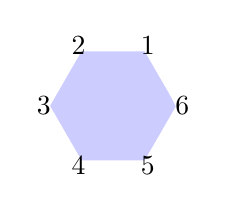
\begin{tikzpicture}
\newdimen\Radi
\Radi=0.8cm
    % Indicate the boundary of the regular polygons
%    \draw [thin,black!20] circle (\R) ;
%    \fill[black!20] circle (2pt);
%    \draw (0:\R) \foreach \x in {120,240} {
%            -- (\x:\R)
%        } -- cycle (90:\R) node[above] {$n=3$} ;
%    \draw[xshift=2.5\R] (0:\R) \foreach \x in {90,180,...,359} {
%            -- (\x:\R)
%        } -- cycle (90:\R) node[above] {$n=4$} ;
%    \draw[xshift=5.0\R] (0:\R) \foreach \x in {72,144,...,359} {
%            -- (\x:\R)
%        } -- cycle (90:\R) node[above] {$n=5$} ;
    \begin{scope}[yshift=-3\Radi]
        \fill[blue!20] (0:\Radi) \foreach \x in {1,...,6} { %60,120,...,359} {
                -- ({60*\x}:\Radi)
            }-- cycle (90:\Radi); % node[above] {$n=6$} ;
        \draw[white] (0:\Radi) \foreach \x in {1,...,6} { %60,120,...,359} {
                -- ({60*\x}:{1.1*\Radi}) node[black] {$\x$}
            }-- cycle (90:\Radi); % node[above] {$n=6$} ;
            
%        % 360/7 = 51.4286 For PGF v < 1.18 we have to round to the nearest
%        % integer. Newer version support fractional angle values.
%        % For a more accurate result use the sequence
%        % {51, 103, 154, 206, 257, 309}
%        %
%        \draw[xshift=2.5\R] (0:\R) \foreach \x in {51.4286,102.8571,...,359} {
%                -- (\x:\R)
%            }-- cycle (90:\R) node[above] {$n=7$} ;
%        \draw[xshift=5.0\R] (0:\R) \foreach \x in {45,90,...,359} {
%                -- (\x:\R)
%            } -- cycle (90:\R) node[above] {$n=8$} ;
    \end{scope}
%    \draw[yshift=-6.0\R] (0:\R) \foreach \x in {10,20,...,359} {
%            -- (\x:\R)
%        } -- cycle (90:\R) node[above] {$n=36$} ;
\end{tikzpicture}
\end{document}

\end{center}
Any symmetry moves \(1\) to one of the six vertices, and moves \(2\) to a next door neighbor vertex.
We can draw the vertices of the hexagon twice, one for drawing where \(1\) is taken to, and once again to represent whether \(2\) is taken to the vertex counterclockwise from \(1\) or clockwise.
\begin{center}
\documentclass[tikz]{standalone}
\begin{document}
% Radius of regular polygons
\begin{tikzpicture}
\newdimen\Radi
\Radi=0.8cm
    % Indicate the boundary of the regular polygons
%    \draw [thin,black!20] circle (\Radi) ;
%    \fill[black!20] circle (2pt);
%    \draw (0:\Radi) \foreach \x in {120,240} {
%            -- (\x:\Radi)
%        } -- cycle (90:\Radi) node[above] {$n=3$} ;
%    \draw[xshift=2.5\Radi] (0:\Radi) \foreach \x in {90,180,...,359} {
%            -- (\x:\Radi)
%        } -- cycle (90:\Radi) node[above] {$n=4$} ;
%    \draw[xshift=5.0\Radi] (0:\Radi) \foreach \x in {72,144,...,359} {
%            -- (\x:\Radi)
%        } -- cycle (90:\Radi) node[above] {$n=5$} ;
        \foreach \x in {1,...,6} { %60,120,...,359} {
                \fill ({\Radi*cos(60*\x)},{\Radi*sin(60*\x)}) circle (1.2pt); % \node{\(b^{\x}c\)};
                \fill ({1.5*\Radi*cos(60*\x)},{1.5*\Radi*sin(60*\x)}) circle (1.2pt); % \node{\(b^{\x}c\)};
		}
            
%        % 360/7 = 51.4286 For PGF v < 1.18 we have to round to the nearest
%        % integer. Newer version support fractional angle values.
%        % For a more accurate result use the sequence
%        % {51, 103, 154, 206, 257, 309}
%        %
%        \draw[xshift=2.5\Radi] (0:\Radi) \foreach \x in {51.4286,102.8571,...,359} {
%                -- (\x:\Radi)
%            }-- cycle (90:\Radi) node[above] {$n=7$} ;
%        \draw[xshift=5.0\Radi] (0:\Radi) \foreach \x in {45,90,...,359} {
%                -- (\x:\Radi)
%            } -- cycle (90:\Radi) node[above] {$n=8$} ;
%    \draw[yshift=-6.0\Radi] (0:\Radi) \foreach \x in {10,20,...,359} {
%            -- (\x:\Radi)
%        } -- cycle (90:\Radi) node[above] {$n=36$} ;
\end{tikzpicture}
\end{document}

\end{center}
In a sense, this is a picture of the group, since every element of the group is completely determined once we know where vertices \(1\) and \(2\) go: the rest are then in order cyclically around the hexagon.
Let \(b\) be rotation of the hexagon by \(60\si{\degree}\), and let \(c\) be reflection of the hexagon across the axis of symmetry through vertex \(1\).
Label the elements of the group according to how they move vertices \(1\) and \(2\), i.e. how much of \(b\) and \(c\) they contain:
\begin{center}
\documentclass[tikz]{standalone}
\usepackage{xparse}
\colorlet{curveZero}{gray!75}
\colorlet{curveOne}{blue!60}
\colorlet{curveTwo}{brown!50!gray}
\colorlet{curveThree}{green!40!gray}
\colorlet{curveFour}{red!50!gray}
\NewDocumentCommand\DrawDotInPlot{O{}mmO{}}%
{%
\fill[gray!20,draw=gray] (axis cs:{#2},{#3}) circle (1.3pt) node[above,black,#4] {\(#1\)};%
}%
\NewDocumentCommand\DrawDot{O{}mmO{}}%
{%
\fill[gray!20,draw=gray] ({#2},{#3}) circle (1.3pt) node[above,black,#4] {\(#1\)};%
}%
\NewDocumentCommand\DrawNode{O{}m}%
{%
\fill[gray!20,draw=gray] (#2) circle (1.3pt) node[above,black] {\(#1\)};%
}%
\colorlet{axisColor}{gray!50}
\tikzstyle{shapeZero}=[fill=curveZero,opacity=.4]
\tikzstyle{shapeOne}=[fill=curveOne,opacity=.4]
\tikzstyle{shapeTwo}=[fill=curveTwo,opacity=.4]
\tikzstyle{shapeThree}=[fill=curveThree,opacity=.4]
\tikzstyle{groupElementLabel}=[minimum size=2.4em]
\tikzstyle{groupElement}=[minimum size=2.4em,shapeZero,draw=curveZero]
\tikzstyle{cosetOne}=[minimum size=2.4em,shapeOne,draw=curveOne]
\tikzstyle{cosetTwo}=[minimum size=2.4em,shapeTwo,draw=curveTwo]


\begin{document}
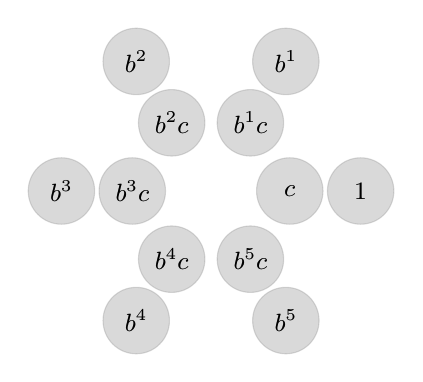
\begin{tikzpicture}
\newdimen\Radi
\Radi=1cm
        \foreach \x in {1,...,5} {
                \node[circle,groupElement] at ({\Radi*cos(60*\x)},{\Radi*sin(60*\x)}) {\small\(b^{\x}c\)};
                \node[circle,groupElementLabel] at ({\Radi*cos(60*\x)},{\Radi*sin(60*\x)}) {\small\(b^{\x}c\)};
                \node[circle,groupElement] at ({1.9*\Radi*cos(60*\x)},{1.9*\Radi*sin(60*\x)}) {\small\(b^{\x}\)};
                \node[circle,groupElementLabel] at ({1.9*\Radi*cos(60*\x)},{1.9*\Radi*sin(60*\x)}) {\small\(b^{\x}\)};
		}
        \node[circle,groupElement] at ({\Radi},{0}) {\small\(c\)};
        \node[circle,groupElementLabel] at ({\Radi},{0}) {\small\(c\)};
        \node[circle,groupElement] at ({1.9*\Radi},{0}) {\small\(1\)};        
        \node[circle,groupElementLabel] at ({1.9*\Radi},{0}) {\small\(1\)};        
\end{tikzpicture}
\end{document}

\end{center}
Multiplication of each element by \(b\) on the left, i.e. \(x \mapsto bx\), spins the hexagon around to right.
\begin{center}
\documentclass[tikz]{standalone}
\begin{document}

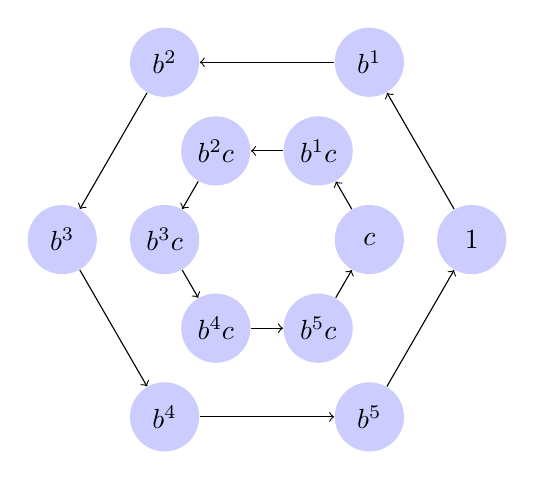
\begin{tikzpicture}
% Radius of regular polygons
\newdimen\Radi
\Radi=1.3cm
        \foreach \x/\n in {1/a,2/b,3/c,4/d,5/e} { 
                \node[circle,minimum size=2.5em,fill=blue!20] ({\n}0) at ({\Radi*cos(60*\x)},{\Radi*sin(60*\x)}) {\(b^{\x}c\)};
                \node[circle,minimum size=2.5em,fill=blue!20] ({\n}1) at ({2*\Radi*cos(60*\x)},{2*\Radi*sin(60*\x)}) {\(b^{\x}\)};
		}
        \node[circle,minimum size=2.5em,fill=blue!20] ({f}0) at ({\Radi},{0}) {\(c\)};
        \node[circle,minimum size=2.5em,fill=blue!20] ({f}1) at ({2*\Radi},{0}) {\(1\)};                  
		\foreach \from/\to in {a/b,b/c,c/d,d/e,e/f,f/a} {
		\draw [->] ({\from}0) -- ({\to}0);
		\draw [->] ({\from}1) -- ({\to}1);
		}
\end{tikzpicture}
\end{document}

\end{center}
Multiplication of each element by \(c\) on the right, i.e. \(x \mapsto xc\), moves the inward hexagon points to the outward ones, and vice versa.
\end{example}

Elements \(g, h, \dots\) of a group \(G\) \emph{generate}\define{generators} that group if every element can be written as a product of integer powers of those elements.
If we fix some elements generating a group \(G\), the \emph{Cayley graph}\define{Cayley graph} of \(G\) (with respect to those generators) is the set of elements of \(G\), each draw as a dot, together with an arrow from one dot to another, labelled by \(g\), if the first dot is some element \(k\) and the second is \(gk\) (or \(kg\), depending on which ordering we prefer).
These pictures are almost never useful in proving results about groups, but they give us some intuition.


Sage knows the Cayley graphs (for various generators) of many groups.
If we type
\begin{sageblock}
H = DihedralGroup(6)
show(H.cayley_graph())
\end{sageblock}
we see the graph:
\begin{center}
\includegraphics[width=5cm]{cayley-graph-d6.png}
\end{center}
The graph is labelled by the cycles of each element, thought of as a permutation of the vertices of the hexagon.

\section{Subgroups}

A subset \(H\) of a group \(G\) is a \emph{subgroup}\define{subgroup} if
\begin{enumerate}
\item
\(H\) contains the identity element and
\item
if \(a\) and \(b\) are elements of \(H\) then \(ab\) is also an element of \(H\), 
\item
if \(b\) is an element of \(H\) then \(b^{-1}\) is also an element of \(H\).
\end{enumerate}

It follows that \(H\) is itself a group.

\begin{example}
The even numbers are a subgroup of the integers, under usual integer addition.
\end{example}
\begin{example}
The invertible integer \(2 \times 2\) matrices are a subgroup of the invertible real \(2 \times 2\) matrices.
\end{example}
\begin{example}
If \(b\) is an element of any group \(G\), then the set of all elements of \(G\) of the form \(b^k\) for integers \(k\) is a cyclic group, the subgroup generated by \(b\).
\end{example}
\begin{example}
The real \(2 \times 2\) matrices of unit determinant form a subgroup of the group of all invertible real \(2 \times 2\) matrices, since determinants multiply.
\end{example}

\section{Cosets}

If \(S\) is any subset of a group \(G\) and \(b\) is any element of \(G\), denote by \(bS\) the set of elements of the form \(bs\) for \(s\) in \(S\), called a \emph{left translate}\define{left translate} or \emph{left coset}\define{left coset} of \(S\); if we write \emph{coset}, we mean \emph{left coset}.
Denote by \(Sb\) the set of elements of the form \(sb\) for \(s\) in \(S\), called a \emph{right translate}\define{right translate} or \emph{right coset}\define{right coset} of \(S\).
Each coset \(bS\) has the same number of elements as \(S\), since \(s \mapsto bs\) has inverse \(t \mapsto b^{-1}t\), so is a bijection.

\begin{example}
The group \(G\) of symmetries of the hexagon has a subgroup \(H\) of rotations of the hexagon.
Divide up \(G\) into \(H\)-cosets:
\begin{center}
\input{hexagon-4}
\end{center}
\end{example}
\begin{example}
We might draw our cosets as columns of a matrix
\begin{center}
\documentclass[tikz]{standalone}
\usepackage{xparse}
\colorlet{curveZero}{gray!75}
\colorlet{curveOne}{blue!60}
\colorlet{curveTwo}{brown!50!gray}
\colorlet{curveThree}{green!40!gray}
\colorlet{curveFour}{red!50!gray}
\NewDocumentCommand\DrawDotInPlot{O{}mmO{}}%
{%
\fill[gray!20,draw=gray] (axis cs:{#2},{#3}) circle (1.3pt) node[above,black,#4] {\(#1\)};%
}%
\NewDocumentCommand\DrawDot{O{}mmO{}}%
{%
\fill[gray!20,draw=gray] ({#2},{#3}) circle (1.3pt) node[above,black,#4] {\(#1\)};%
}%
\NewDocumentCommand\DrawNode{O{}m}%
{%
\fill[gray!20,draw=gray] (#2) circle (1.3pt) node[above,black] {\(#1\)};%
}%
\colorlet{axisColor}{gray!50}
\tikzstyle{shapeZero}=[fill=curveZero,opacity=.4]
\tikzstyle{shapeOne}=[fill=curveOne,opacity=.4]
\tikzstyle{shapeTwo}=[fill=curveTwo,opacity=.4]
\tikzstyle{shapeThree}=[fill=curveThree,opacity=.4]
\tikzstyle{groupElementLabel}=[minimum size=2.4em]
\tikzstyle{groupElement}=[minimum size=2.4em,shapeZero,draw=curveZero]
\tikzstyle{cosetOne}=[minimum size=2.4em,shapeOne,draw=curveOne]
\tikzstyle{cosetTwo}=[minimum size=2.4em,shapeTwo,draw=curveTwo]


\begin{document}
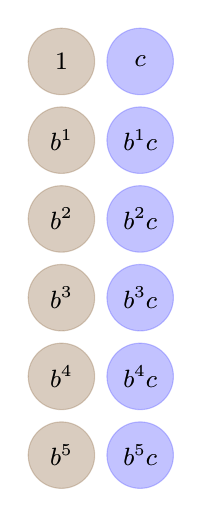
\begin{tikzpicture}
\newcommand{\Radx}{1}
        \foreach \x in {1,...,5} {
                \node[circle,cosetOne] 
                at (1,{-\Radx*\x}) 
                {\small\(b^{\x}c\)};
                \node[circle,groupElementLabel] 
                at (1,{-\Radx*\x}) 
                {\small\(b^{\x}c\)};
                \node[circle,cosetTwo] 
                at (0,{-\Radx*\x}) 
                {\small\(b^{\x}\)};
                \node[circle,groupElementLabel] 
                at (0,{-\Radx*\x}) 
                {\small\(b^{\x}\)};
		}
        \node[circle,cosetOne] 
        at (1,0) 
        {\small\(c\)};
        \node[circle,groupElementLabel] 
        at (1,0) 
        {\small\(c\)};
        \node[circle,cosetTwo] 
        at (0,0) 
        {\small\(1\)};        
        \node[circle,groupElementLabel] 
        at (0,0) 
        {\small\(1\)};        
\end{tikzpicture}
\end{document}

\end{center}
to emphasize that they are all the same size, each a copy of \(H\).
\end{example}
\begin{example}
Let \(G\) be the group of rotations and \(H\) the subgroup of those rotations which preserve a regular hexagon \(X\) around the origin.
For each angle \(\theta\), which we think of as a rotation \(g\), \(gH\) is the set of all rotations \(gh\) for \(h \in H\), i.e. geometrically the rotations which take the given hexagon \(X\) into the hexagon \(gX\).
\end{example}
\begin{example}
Let \(G\) be the group of integers under addition, and \(H\) the subgroup of multiples of \(7\), i.e. \(H\) is the set of all integers of the form \(7k\) for any integer \(k\).
Our translates in this notation have the form \(1+H, 2+H\), and so on.
The translate \(1+H\) is the set of all numbers of the form \(1+7k\) for any integer \(k\).
The translate \(2+H\) is the set of all numbers of the form \(2+7k\) for any integer \(k\), and so on.
\end{example}

\begin{lemma}\label{lemma:coset.id}
If \(x\) and \(y\) are elements of a group \(G\) and \(H\) is a subgroup of \(G\), then \(xH=yH\) just when \(y^{-1}x\) belongs to \(H\).
Any two cosets \(xH\) and \(yH\) are either disjoint: \(xH \cap yH\) empty, or equal: \(xH=yH\).
\end{lemma}
\begin{proof}
Suppose that \(xH=yH\).
Then every element \(xh\) of \(xH\) must belong to \(yH\), i.e. have the form \(yh'\) for some element \(h'\) of \(H\), so \(xh=yh'\), i.e. \(x=yh'h^{-1}\), and so \(y^{-1}x=h'h^{-1}\) is in \(H\).

Conversely, if \(y^{-1}x\) is in \(H\), then every element \(xh\) of \(xH\) has the form
\begin{align*}
xh
&=
(yy^{-1})xh, \\
&=
y(y^{-1}xh),
\\
&= yh'
\end{align*}
where \(h' = y^{-1}xh\) is in \(H\).
Similarly, every element \(yh\) of \(yH\) has the form
\begin{align*}
yh
&=
(xx^{-1})xh, \\
&=
x(x^{-1}yh),
\\
&= xh'
\end{align*}
where \(h' = x^{-1}yh = (y^{-1}x)^{-1}h\) is in \(H\).

If \(xH\) intersects \(yH\), say at \(xh=yh'\), then \(y^{-1}xh=h'\) lies in \(H\) so \(y^{-1}x\) lies in \(H\), i.e. \(xH=yH\).
\end{proof}


If \(H\) is a subgroup of a group \(G\), we let \(G/H\) be the collection of all cosets of \(H\) in \(G\).

\begin{example}
The group \(G\) of symmetries of the hexagon has a subgroup \(H\) of rotations of the hexagon.
If we  draw each coset as a column, we draw each point of \(G/H\) as a single dot underneath that column:
\begin{center}
\documentclass[tikz]{standalone}
\begin{document}

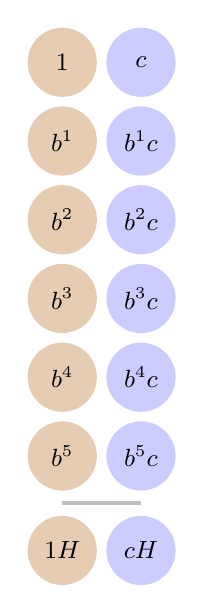
\begin{tikzpicture}
\newcommand{\Radiii}{1}
        \foreach \x in {1,...,5} {
                \node[circle,minimum size=2.5em,fill=blue!20] at (1,{-\Radiii*\x}) {\small\(b^{\x}c\)};
                \node[circle,minimum size=2.5em,fill=brown!40] at (0,{-\Radiii*\x}) {\small\(b^{\x}\)};
		}
        \node[circle,minimum size=2.5em,fill=blue!20] at (1,0) {\small\(c\)};
        \node[circle,minimum size=2.5em,fill=brown!40] at (0,0) {\small\(1\)};        
        \draw [gray!50,ultra thick] (0,{-\Radiii*5.6}) -- (1,{-\Radiii*5.6});
        \node[circle,minimum size=2.5em,fill=blue!20] at (1,{-\Radiii*6.2}) {\small\(cH\)};
        \node[circle,minimum size=2.5em,fill=brown!40] at (0,{-\Radiii*6.2}) {\small\(1H\)};        
        
\end{tikzpicture}
\end{document}

\end{center}
\end{example}
\begin{example}
Let \(G\) be the group of all rotations of the plane and \(H\) the subgroup of those rotations which preserve a regular hexagon \(X\) around the origin.
For each angle \(\theta\), which we think of as a rotation \(g\), \(gH\) is the set of all rotations \(gh\) for \(h \in H\), i.e. geometrically the rotations which take the given hexagon \(X\) into the hexagon \(gX\).
So each coset \(gH\) in \(G/H\) is identified with a rotated hexagon \(gX\), i.e. \(G/H\) is the set of all rotated hexagons \(gX\) for any rotation \(g\).
\end{example}
\begin{example}
Let \(G\) be the group of integers under addition, and \(H\) the subgroup of multiples of \(7\), i.e. \(H\) is the set of all integers of the form \(7k\) for any integer \(k\).
Our translates in this notation have the form \(1+H, 2+H\), and so on.
The translate \(1+H\) is the set of all numbers of the form \(1+7k\) for any integer \(k\), which we denote by \(\bar{1}\).
The translate \(2+H\) is the set of all numbers of the form \(2+7k\) for any integer \(k\), which we denote by \(\bar{2}\), and so on.
Of course, \(\bar{7}=\bar{0}\) is the coset of \(H\).
So \(G/H\) is the set of remainders modulo \(7\).
Each element of \(G/H\) represents ``gluing together'' all elements of \(G\) that differ by a multiple of \(H\).
\end{example}

\section{Actions}

A group \(G\) \emph{acts} on a set \(X\) if each element \(b\) of \(G\) has an associated transformation \(f_g\) of \(X\)  so that \(f_{bc} = f_b \circ f_c\) for any elements \(b, c\) of \(G\).
So then \(G\) is a transformation group of \(X\), and write \(gx\) to mean \(f_g(x)\).
The action is \emph{transitive} if any two points \(p, q\) of \(X\) are connected by some element of \(G\), i.e. \(q=gp\) for some \(g\) in \(G\).
The \emph{stabilizer} of a point \(x_0\) of \(X\) is the subset \(G^{x_0}\) of \(G\) consisting of those \(g\) in \(G\) so that \(gx_0=x_0\).
If a group \(G\) acts on two sets \(X\) and \(Y\), a map \(f \colon X \to Y\) is \emph{equivariant} if \(f(gx)=gf(x)\) for any \(x\) in \(X\) and \(g\) in \(G\).
An equivariant bijection makes two actions practically identical.

\begin{lemma}
Given a group action of a group \(G\) on a set \(X\), and an element \(x_0\) of \(X\), the stabilizer \(G^{x_0}\) of each point is a subgroup.
\end{lemma}
\begin{proof}
Clearly if \(bx_0=x_0\) and \(cx_0=x_0\) then \((bc)x_0=b(cx_0)=bx_0=x_0\) and so on.
\end{proof}

Subgroups correspond to transitive actions; geometrically it is always easier to think about actions, but algebraically it is easier to work with subgroups.
\begin{theorem}
If \(H\) is a subgroup of a group \(G\), and we let \(X=G/H\), then \(G\) acts on \(X\) transitively by \(b(cH)=(bc)H\) with stabilizer \(G^{x_0}=H\) where \(x_0\) is the coset \(1H\).
Conversely, if \(G\) acts transitively on a set \(X\), and we let \(H=G^{x_0}\), there is a unique equivariant bijection
\(
f \colon G/H \to X,
\)
so that \(f(gH)=gx_0\).
\end{theorem}
\begin{proof}
Clearly \(b(cH)=(bc)H\) is the set of elements of \(G\) of the form \(bch\) for \(h\) in \(H\).
Hence the action of \(G\) on \(G/H\) is defined.

Take any element \(gH\) of \(G/H\).
So \(gH\) is a coset.
By lemma~\vref{lemma:coset.id}, knowing only the coset \(gH\), we can determine the element \(g\), up to replacing \(g\) by \(gh\) for any \(h \in H\).
But then the expression \(gx_0\) will only change to \((gh)x_0=g(hx_0)=gx_0\), i.e. not at all.
So knowledge of the coset \(gH\) determines knowledge of \(gx_0\), i.e. \(f\) is well defined.
It is then easy to check that \(f\) is equivariant.
Since \(G\) acts transitively on \(X\), every element \(x\) of \(X\) has the form \(x=gx_0\) for some \(g\), \(f\) is surjective.
If \(f(bH)=f(cH)\) then \(bx_0=cx_0\) so \(c^{-1}bx_0 = x_0\) i.e. \(c^{-1} b\) lies in \(G^{x_0}\).
But \(H\) is by definition \(G^{x_0}\), so \(c^{-1}b\) lies in \(H\), i.e. \(bH=cH\), so \(f\) is injective.
\end{proof}



\begin{theorem}[Lagrange]\SubIndex{Lagrange, Joseph-Louis}
If \(H\) is a finite subgroup of a group \(G\) then
\[
|G/H|=\frac{|G|}{|H|}.
\]
\end{theorem}
\begin{proof}
The set \(G\) is divided up into disjoint cosets, each containing \(|H|\) elements.
\end{proof}


\begin{corollary}
The order of any finite subgroup of a group divides the order of the group.
\end{corollary}

\begin{corollary}
The order of any element of a group divides the order of the group.
\end{corollary}

\begin{corollary}
Every finite group of prime order, say order \(p\), is cyclic, isomorphic to the group of remainders modulo \(p\) under addition.
\end{corollary}
\begin{proof}
Take any element which is not the identity element, so cannot have order 1.
Since \(G\) is finite, the order of the element is finite.
Since \(|G|\) is prime, the order of the element divides this prime, so equals this prime.
\end{proof}


Take a group \(G\) acting on a set \(X\).
The \emph{orbit}\define{orbit} \(Gx\) of an element \(x\) of \(X\) is the set of all elements of \(X\) of the form \(gx\) for \(g\) in \(G\): it is where \(G\) takes \(x\).
Every orbit is, by definition, acted on transitively by \(G\), so the map \(G/G^x \to Gx\) taking \(gG^x \mapsto gx\) is an equivariant bijection.

\begin{problem}{groups:orbits.square}
If \(X\) is a hexagon in the plane, and \(G\) is the symmetry group of \(X\), what are all of the orbits of \(G\)?
\end{problem}

A \emph{fixed point}\define{fixed point} of a group \(G\) acting on a set \(X\) is a point \(x\) fixed by all elements of \(G\), i.e. \(gx=x\) for any \(g\) in \(G\).

\begin{problem}{groups:fixed.point}
If a finite group \(G\) acts on a finite set \(X\), and the order of \(X\) is coprime to the order of \(G\), prove that \(X\) contains a fixed point of the \(G\)-action.
\end{problem}



\section{Group presentations}

\begin{example}
The symmetries of an equilateral triangle can all be expressed in terms of the rotation, call it \(b\), by \(120\si{\degree}\), and the reflection, call it \(c\), about any one the axes of symmetry through one of the vertices.
Clearly \(b^3=1\), i.e. if we rotate three times by \(120\si{\degree}\), the resulting rotation by \(360\si{\degree}\) moves every point back where it started.
Similarly \(c^2=1\).
The reader can draw pictures to see that \(bc=cb^2\).
Once we have these three rules, any expression in the group in terms of \(b\) and \(c\) can be successively simplified by these three rules, to an expression in which \(c\) only appears to the first power, i.e. no \(c^2\) or \(c^{-1}\) or \(c^{-13}\) appears, and \(b\) appears only to the power \(1\) or \(2\), and \(b\) always appears after \(c\).
Hence the group is precisely
\[
1,b,c,b^2,cb,cb^2.
\]
\end{example}


Take an abstract set \(S\).
A \emph{word}\define{word} on the \emph{alphabet}\define{alphabet} \(S\) is a finite sequence of choices of element of \(S\) and integer power.
We write each word as a string of symbols
\[
s_1^{a_1} s_2^{a_2} \dots s_k^{a_k}.
\]
We allow the empty string, and write it as \(1\).
\emph{Reduce}\define{reduce} a word by deleting any \(s^0\) symbols and replacing any subword \(s^p s^q\) by \(s^{p+q}\).
The \emph{free group}\define{free!group} \(\left<S\right>\) on an alphabet \(S\) is the collection of all reduced words on \(S\).
The multiplication operation: multiply two words by writing down one after the other, called \emph{concatenation}\define{concatentation} and then reducing.
The inverse operation: write down the word in reverse order, with opposite signs for the powers.

Take an abstract set \(S\) with associated free group \(\left<S\right>\).
Take a subset \(R \subset \left<S\right>\).
The group \emph{generated} by \(S\) with \emph{relations} \(R\), denoted \(\left<S|R\right>\), is the quotient of \(\left<S\right>\) by the smallest normal subgroup containing \(R\).
The expression of a group in the form \(\left<S|R\right>\) is a \emph{presentation}\define{presentation} of the group with \emph{generators} \(S\) and \emph{relations} \(R\).

\begin{lemma}
Every map of sets \(f \colon S \to G\) to a group extends uniquely to a morphism of groups \(f \colon \left<S\right> \to G\).
It therefore extends to an injective morphism of groups \(\left<S|R\right> \to G\) where \(R\) is the set of all words 
\[
w=s_1^{a_1} s_2^{a_2} \dots s_k^{a_k}
\]
on the alphabet \(S\) for which
\[
f(s_1)^{a_1} \dots f(s_k)^{a_k} = 1.
\]
\end{lemma}

In practice, we usually write the relations not as a set \(R\), but as a collection of equations like
\[
w_1 = w_2
\]
between words.
This equation means that we require \(w_2^{-1} w_1 \in R\).

\begin{example}
The two transformations
\[
T \colon (x,y) \mapsto (x,y+1)
\]
and
\[
F \colon (x,y) \mapsto (x+1,-y)
\]
of the plane, a translation and a flip, satisfy \(TFT=F\), and generate some group \(H\), the symmetries of the wallpaper pattern:
\begin{center}
\includegraphics[width=4cm]{Wallpaper_group-pg-1.jpg}
\end{center}
Let \(G \defeq \left<f,t|tft=f\right>\); in other words \(G\) is the group generated by alphabet \(\set{t,f}\) with relation \(tft=t\), i.e. with \(R=\set{t^{-1}tft}\).
So we have a surjective map
\(
G \to H
\),
mapping \(t \mapsto T\) and \(f \mapsto F\).
Here \(t\) is a formal symbol, not an actual transformation of the plane, while \(T\) is the actual transformation.
Take any word in \(G\).
Wherever we find \(tf\) we replace it by \(ft^{-1}\).
Wherever we find \(t^{-1}f\) we replace it by \(ft\).
Wherever we find \(tf^{-1}\) we replace it by \(f^{-1}t^{-1}\).
Wherever we find \(t^{-1}f^{-1}\) we replace it by \(f^{-1}t\).
The reader can check that these are all consequences of \(tft=f\).
Therefore any word in \(G\) can be written uniquely as \(f^p t^q\).
If the corresponding transformation \(F^p T^q\) is the identity, then it fixes the origin, and so the translations of the \(x\) variable cancel each other out, i.e. \(p=0\).
But then \(T^q(x,y)=(x,y+q)\) fixes the origin just when \(q=0\).
So the only element of \(G\) mapping to the trivial transformation of the plane is \(1\).
We can see that \(G \to H\) is an isomorphism.
\end{example}



\section{Morphisms}

A \emph{morphism}\define{morphism!of groups} of groups is a map \(\phi \colon G \to H\) so that \(\phi(xy)=\phi(x)\phi(y)\): \(\phi\) preserves multiplication. 
We have seen several of these.
\begin{example}
Label the vertices of an equilateral triangle as \(1,2,3\).
Identify the group \(G\) of symmetries of the triangle with the symmetric group \(H\) on 3 letters, by taking each symmetry \(g\) of the equilateral triangle to the permutation \(h=\phi(g)\) of its vertices.
\end{example}
\begin{example}
Label the vertices of any polygon \(X\) in the plane, or polyhedron \(X\) in Euclidean 3-dimensional space, with \(n\) vertices.
Map the group \(G\) of symmetries of \(X\) to the symmetric group \(H\) on \(n\) letters, by taking each symmetry \(g\) of \(X\) to the permutation \(h=\phi(g)\) of its vertices.
This map might not be surjective.
For example, if \(X\) is a square in the plane
\begin{center}
\documentclass[tikz]{standalone}
\usepackage{xparse}
\usetikzlibrary{positioning}
\colorlet{curveZero}{gray!75}
\colorlet{curveOne}{blue!60}
\colorlet{curveTwo}{brown!50!gray}
\colorlet{curveThree}{green!40!gray}
\colorlet{curveFour}{red!50!gray}
\NewDocumentCommand\DrawDotInPlot{O{}mmO{}}%
{%
\fill[gray!20,draw=gray] (axis cs:{#2},{#3}) circle (1.3pt) node[above,black,#4] {\(#1\)};%
}%
\NewDocumentCommand\DrawDot{O{}mmO{}}%
{%
\fill[gray!20,draw=gray] ({#2},{#3}) circle (1.3pt) node[above,black,#4] {\(#1\)};%
}%
\NewDocumentCommand\DrawNode{O{}m}%
{%
\fill[gray!20,draw=gray] (#2) circle (1.3pt) node[above,black] {\(#1\)};%
}%
\colorlet{axisColor}{gray!50}
\tikzstyle{shapeZero}=[fill=curveZero,opacity=.4]
\tikzstyle{shapeOne}=[fill=curveOne,opacity=.4]
\tikzstyle{shapeTwo}=[fill=curveTwo,opacity=.4]
\tikzstyle{shapeThree}=[fill=curveThree,opacity=.4]
\tikzstyle{groupElementLabel}=[minimum size=2.4em]
\tikzstyle{groupElement}=[minimum size=2.4em,shapeZero,draw=curveZero]
\tikzstyle{cosetOne}=[minimum size=2.4em,shapeOne,draw=curveOne]
\tikzstyle{cosetTwo}=[minimum size=2.4em,shapeTwo,draw=curveTwo]


\newcounter{squareBoxCounter}
\begin{document}
\setcounter{squareBoxCounter}{0}
\NewDocumentCommand\sqrbox{mmmm}{%
\stepcounter{squareBoxCounter}%
\begin{scope}[xshift=\thesquareBoxCounter in]%
\fill[shapeZero,draw=curveZero] (0,0) rectangle (1,1);%
\node[below left=-1.3mm and -1.3mm] at (0,0) {#1};%
\node[above left=-1.3mm and -1.3mm] at (0,1) {#2};%
\node[above right=-1.3mm and -1.3mm] at (1,1) {#3};%
\node[below right=-1.3mm and -1.3mm] at (1,0) {#4};%
\end{scope}}%
\begin{tikzpicture}[scale=.5]%
\sqrbox{1}{2}{3}{4}%
\sqrbox{4}{1}{2}{3}%
\sqrbox{1}{4}{3}{2}%
\end{tikzpicture}%
\end{document}
\end{center}
no rotation or reflection will ever put \(1\) and \(2\) diagonally across from each other, because that would pull them apart to a greater distance.
\end{example}
\begin{example}
Every element \(g\) of any group \(G\) has associated a morphism
\[
\phi \colon \Z{} \mapsto G,
\]
given by \(\phi(k)=g^k\).
This map is surjective just when \(G\) is cyclic, and injective just when \(g\) has infinite order.
\end{example}

Almost everything we know about any group arises from looking at morphisms to that group and from that group.
The \emph{kernel}\define{kernel} of a morphism \(\phi \colon G \to H\) is the set of all elements \(g\) of \(G\) for which \(\phi(g)=1\), i.e. the elements ``killed'' by \(\phi\).
The \emph{image}\define{image} of a morphism \(\phi \colon G \to H\) is the set of all elements \(h\) of \(H\) for which \(h=\phi(g)\) for some \(g\) in \(G\).

\begin{problem}{groups:kernel}
Prove that the kernel of any morphism of groups \(\phi \colon G \to H\) is a subgroup of \(G\).
\end{problem}

\begin{problem}{groups:kernel.2}
Prove that the kernel of any morphism of groups \(\phi \colon G \to H\) is \(\set{1}\) just when \(\phi\) is injective.
\end{problem}

\begin{problem}{groups:image}
Prove that the image of any morphism of groups \(\phi \colon G \to H\) is a subgroup of \(H\).
\end{problem}

It seems natural to ask which subgroups arise as kernels and as images.

\begin{problem}{groups:image.2}
Prove that every subgroup \(G\) of any group \(H\) is the image of a morphism of groups \(\phi \colon G \to H\).
\end{problem}

A subgroup \(K\) of a group \(G\) is \emph{normal} if \(gKg^{-1}=K\) for any \(g\) in \(G\).

\begin{problem}{groups:rigid.motion.normal}
Every rigid motion \(f\) of three dimensional Euclidean space can be written uniquely as \(f(x)=Ax+b\) where \(A\) is an orthogonal matrix and \(b\) is a vector in three dimensional Euclidean space.
A \emph{translation} is a rigid motion \(f\) of the form \(f(x)=x+b\).
An \emph{orthogonal transformation} is a rigid motion \(f\) of the form \(f(x)=Ax\).
Let \(G\) be the group of all rigid motions three dimensional Euclidean space.
Let \(T\) be the set of all translations.
Prove that \(T\) is a normal subgroup of \(G\).
Let \(U\) be the set of all orthogonal transformations.
Prove that \(U\) is \emph{not} a normal subgroup of \(G\).
\end{problem}

\begin{theorem}
A subset \(K\) of a group \(G\) is a normal subgroup if and only if \(K\) is the kernel of some morphism \(\phi \colon G \to H\) to some group \(H\).
Indeed, if \(K\) is normal, then there is a unique group operation on \(G/K\) so that the map \(\phi \colon G \to G/K\) given by \(\phi(g)=gK\) is a group morphism with kernel \(K\).
\end{theorem}
\begin{proof}
If \(K\) is the kernel of a morphism \(\phi \colon G \to H\) to some group \(H\), then an element \(k\) of \(G\) belongs to \(K\) just when \(\phi(k)=1\).
But 
\[
\phi(gkg^{-1})
=
\phi(g)\phi(k)\phi(g)^{-1}
\]
so \(\phi(k)=1\) implies \(\phi(gkg^{-1})=1\) i.e. if \(k\) lies in \(K\) then \(gkg^{-1}\) does too.
Similarly,
\begin{align*}
\phi(k)
&=
\phi(g^{-1}g \, k \, g^{-1}g),
\\
&=
\phi(g)^{-1}\phi(g \, k \, g^{-1})\phi(g),
\end{align*}
so \(\phi(gkg^{-1})=1\) implies \(\phi(k)=1\) i.e. \(k\) lies in \(K\) just when \(gkg^{-1}\) does too.
Hence \(K\) is normal.

Suppose that \(K\) is normal.
Define on \(G/K\) the operation \((bK)(cK)=bcK\).
It is convenient to write each coset \(bK\) of \(K\) as \(\bar{b}\).
Then the operation is \(\bar{b}\bar{c}=\overline{bc}\), with identity \(\bar{1}\).
To see that this is well defined, note that knowledge of the coset \(bK\) determines \(b\) precisely up to replacing \(b\) by \(bk\) for some \(k\) in \(K\).
Hence \(\bar{b}\) determines \(b\) uniquely up to the equation \(\bar{b}=\overline{bk}\) for \(k\) in \(K\).
So given \(\bar{b}\) and \(\bar{c}\), we know \(b\) and \(c\) precisely up to replacing them with \(bk_0\) and \(ck_1\) for some \(k_0, k_1\) in \(K\).
Hence this replaces \(bc\) by
\[
bk_0 ck_1 = bc (c^{-1} k_0 c) k_1.
\]
But then taking \(K\)-cosets,
\[
\overline{bk_0 ck_1} = \overline{bc}.
\]
Hence the resulting product \(\bar{bc}\) comes out the same for \(b,c\) and for \(bk_0\) and \(ck_1\), i.e. the operation is well defined.
The kernel of this operation is the set of elements \(b\) of \(G\) for which \(\bar{b}=\bar{1}\) i.e. \(bK=K\) i.e. \(b\) in \(K\).
\end{proof}

Sage can tell you whether the subgroup \(H\) generated by some elements \(r_1,r_2,r_3\) is a normal subgroup:
\begin{sageblock}
A4 = AlternatingGroup(4)
r1 = A4("(1,2) (3,4)")
r2 = A4("(1,3) (2,4)")
r3 = A4("(1,4) (2,3)")
H = A4.subgroup([r1, r2, r3])
H.is_normal(A4)
\end{sageblock}
yields \(\sage{H.is_normal(A4)}\).

\begin{theorem}
The image of any morphism of groups \(\phi \colon G \to H\) with kernel \(K\) is isomorphic to \(G/K\) by the isomorphism
\[
\bar\phi \colon G/K \to H
\]
given by \(\bar\phi(gK)=\phi(g)\).
If \(\phi\) is onto, then \(\bar\phi\) is onto.
\end{theorem}
\begin{proof}
When we map \(g\) to \(\phi(g)\), if we replace \(g\) by \(gk\) for any \(k\) in \(K\), this replaces \(\phi(g)\) by \(\phi(gk)=\phi(g)\phi(k)=\phi(g)1=\phi(g)\).
Hence \(\bar\phi(\bar{g})=\phi(g)\) is well defined.
It is morphism of groups because \(\bar\phi(\overline{bc})=\phi(bc)=\phi(b)\phi(c)=\bar\phi(\bar{b})\bar\phi(\bar{c})\).
Its kernel is \(\set{\bar{1}}\), because \(\bar\phi(\bar{b})=1\) just when \(\phi(b)=1\) just when \(b\) is in \(K\), so just when \(\bar{b}=\bar{1}\) is the identity element of \(G/K\).
\end{proof}

Sage knows how to construct the quotient group \(G/H\):
\begin{sageblock}
A4 = AlternatingGroup(4)
r1 = A4("(1,2) (3,4)")
r2 = A4("(1,3) (2,4)")
r3 = A4("(1,4) (2,3)")
H = A4.subgroup([r1, r2, r3])
A4.quotient(H)
\end{sageblock}
yields \(\sage{A4.quotient(H)}\), meaning that the quotient group is isomorphic to the group of permutations generated by the cycle \((1 \ 2 \ 3)\).


\begin{lemma}
Suppose that \(\phi \colon G \to H\) is a morphism of groups and that \(N_G\) and \(N_H\) are normal subgroups of \(G\) and \(H\) and that \(\phi(N_G)\) lies in \(N_H\).
Then there is a unique morphism \(\bar\phi \colon G/N_G \to H/N_H\) so that \(\bar\phi(gN_G)=\phi(g)N_H\).
\end{lemma}
\begin{proof}
If we replace \(g\) by \(gn\) for some \(n\) in \(N_G\), then we alter \(\phi(g)\) to \(\phi(gn)=\phi(g)\phi(n)\).
So we don't change \(\phi(g)N_H\).
Hence \(\bar\phi\) is defined.
It is easy to check that \(\bar\phi\) is a morphism of groups.
\end{proof}

\begin{problem}{groups:action.kernel}
The \emph{kernel} \(K\) of the action of a group \(G\) on a set \(X\) is the set of elements \(g\) of \(G\) so that \(gx=x\) for every \(x\) in \(X\), i.e. the kernel is the set of elements that act trivially.
Prove that the kernel of any action is a normal subgroup, and that there is a unique action of \(G/K\) on \(X\) so that \((gK)x=gx\) for any \(g\) in \(G\) and \(x\) in \(X\).
\end{problem}


\begin{theorem}
Suppose that \(N\) is a normal subgroup of a group \(G\) and lies inside another normal subgroup \(H\) of \(G\).
Then \(G/H\) is isomorphic to \((G/N)/(H/N)\) via the map \(f(gH)=(gN)(H/N)\).
\end{theorem}
\begin{proof}
Note that \(H/N\) is a  normal subgroup of \(G/N\) because its elements are \(hN\) for \(h\) in \(H\) and so, for any \(gN\) in \(G/N\), so
\[
(gN)(hN)(gN)^{-1}=(gN)(hN)(g^{-1}N)=ghg^{-1}N
\]
lies in \(H/N\).
Therefore by the above result, the surjective morphism \(\phi \colon G \to G/N\) descends to a surjective morphism \(\bar\phi \colon G/H \to (G/N)/(H/N)\). 
The kernel of this morphism consist of the \(gH\) so that \(\phi(g)\) lies in \(H/N\), i.e. \(g\) lies in \(H\), i.e. \(gH=H\) is the identity element.
\end{proof}


\section{Amalgamations}

Suppose that \(G\) and \(H\) are two groups.
We would like to define a group \(G*H\), which contains \(G\) and \(H\), and is otherwise ``as unconstrained as possible''.
The product \(G \times H\) is not ``unconstrained'', because the elements of \(G\) commute with those of \(H\) inside \(G \times H\).

First, note that any group \(G\) has an obvious group morphism \(\left<G\right> \to G\) given by \(g \mapsto g\).
It will help to write out concatenations using some symbol like
\[
g_1 * g_2 * \dots * g_n \in \left<G\right>.
\]
Then we can write our group morphism as
\[
g_1 * g_2 * \dots * g_n \in \left<G\right> \mapsto g_1 g_2 \dots g_n \in G.
\]
This group morphism is clearly surjective, with kernel precisely the group \(N_G \subset \left<G\right>\) whose elements are the concatenations
\[
g_1 * g_2 * \dots * g_n
\]
for which \(g_1 g_2 \dots g_n=1\).
So we can write
\[
G=\left<G|N_G\right>.
\]
Think of \(N_G\) as encoding all of the equations satisfied inside the group \(G\).

The \emph{free product}\define{free!product} \(G*H\)\Notation{G*H}{G*H}{amalgation} to be the group \(\left<G \sqcup H|N_G \sqcup N_H\right>\) generated by the elements of \(G\) and \(H\), subject to the relations consisting of all equations satisfied by elements of \(G\) together with all equations satisfied by elements of \(H\).

Another way to look at this: a \emph{word}\define{word} in \(G,H\) is a finite sequence of elements of \(G\) and of \(H\) (perhaps empty), written beside one another with \(*\) symbols inbetween, like
\[
g_1 * g_2 * h_1 * g_3 * h_2 * h_3 * g_4,
\]
et cetera.
We denote the empty sequence as \(1\).
We \emph{reduce} a word by deleting any appearance of the identity element (of either group), and also by replacing any two neighboring elements from the same group by their product in that group:
\[
g_1 * g_2 \mapsto g_1 g_2.
\]
A word is \emph{reduced} if we cannot further reduce it.
The group \(G*H\) is the set of reduced words, with multiplication being simply writing down one word after another and then reducing.

A further wrinkle: suppose that \(K \subset G\) is a subgroup which also appears as a subgroup of \(H\): \(K \subset H\).
The \emph{amalgamation} of \(G\) and \(H\) over \(K\), denoted \(G*_K H\),\Notation{G*KH}{G*_K H}{amalgation over a subgroup}, is
\[
G *_K H = \left<G \sqcup H|N_G \sqcup N_H \sqcup E\right>
\]
where \(E\) is the collection of equations \(k_G=k_H\) where \(k_G\) is an element of \(K\) as a subgroup of \(G\), and \(k_H\) is the associated element of \(K \subset H\).

